\documentclass[russian,utf8,simple]{eskdtext}

% packages
%
% Тестовое наполнение текстом
% При написании работы - удалить пакет и комманды \lipsum
\usepackage{lipsum}
%
\usepackage{graphicx}
\usepackage{datetime}
\usepackage{lastpage} % Number of pages
\usepackage{hyperref} % Links in pdf

% setup
\newcommand{\FrontPageDepartment}{ИТ} %Факультет
\newcommand{\FrontPageSubdepartment}{ИС} %Кафедра
\newcommand{\WorkType}{Курсовой проект} %Тип работы (заголовок)
\newcommand{\Subject}{Предмет} %по ... родительный падеж
\newcommand{\Topic}{Тема курсового проекта} %Тема
\newcommand{\Professor}{Иванов~И.~И.} %Руководитель
\newcommand{\Student}{Петров~П.~П.} %Студент
\newcommand{\Group}{ИСм-112} %Группа
\newcommand{\FrontPageDate}{\ddmmyyyydate\today} %Дата

\ESKDsignature{МИВУ 230400.68 ПЗ} % Код специальности и тип работы

% eskdx setup
\ESKDletter{}{У}{}
\ESKDtitle{\Topic}
\ESKDchecker{\Professor}
\ESKDauthor{\Student}
\ESKDcolumnIX{МИ ВлГУ\\ \Group}

\addto\captionsrussian{\def\refname{Список использованных источников}}
\graphicspath{{img/}} % path to directory with images
\sloppy % split long lines

% verbatim setup
\newcommand{\verbatimFont}{
\fontsize{10pt}{12pt}\selectfont
\baselineskip=1em
}

% main document
\begin{document}
% Титул
\newlength{\frontpagefk} % Ширина поля Факультет/Кафедра
\setlength{\frontpagefk}{6cm}
\newlength{\frontpagerb} % Ширина надписей Руководитель/Студент и пр. под темой
\setlength{\frontpagerb}{6cm}
\newlength{\frontpagerbspace} % ??? (do not remove)
\setlength{\frontpagerbspace}{1cm}
\newlength{\FrontPageSubjSpace} % Ширина пробела до и после названия предмета
\setlength{\FrontPageSubjSpace}{1cm}
\newlength{\FrontPageTopicSpace} % Ширина пробела до и после темы
\setlength{\FrontPageTopicSpace}{0.5cm}

\thispagestyle{empty}
\begin{center}
{
\vspace*{-1.5cm}
\baselineskip=1.3em
{\small Министерство образования и науки Российской Федерации}\\
\textbf{Муромский институт (филиал)}\\
{\footnotesize федерального государственного бюджетного образовательного учреждения\\
высшего профессионального образования}\\
\textbf{<<Владимирский государственный университет\\
имени Александра Григорьевича и Николая Григорьевича\\
Столетовых>>\\
(МИ (филиал) ВлГУ)\\}
}

\bigskip
\begin{tabular}{l c}
\textbf{Факультет}&\underline{\makebox[\frontpagefk]{\FrontPageDepartment}}\\
\textbf{Кафедра}&\underline{\makebox[\frontpagefk]{\FrontPageSubdepartment}}\\
\end{tabular}

\vspace{\fill}
\begin{Huge}
\textbf{\textsl{\WorkType}}
\end{Huge}

\vspace{\fill}
по\underline{\makebox[\FrontPageSubjSpace]{}\Subject\makebox[\FrontPageSubjSpace]{}}

\smallskip
Тема:\underline{\makebox[\FrontPageTopicSpace]{}\Topic\makebox[\FrontPageTopicSpace]{}}

\vspace{\fill}

\begin{flushright}
\makebox[\frontpagerb][c]{
\makebox[\frontpagerb][l]{Руководитель}\hspace{\frontpagerbspace}}

\smallskip
\makebox[\frontpagerb][c]{
\raisebox{-\baselineskip}{\shortstack{\underline{\makebox[\frontpagerb][l]{\Professor}}\\
\begin{footnotesize}
(фамилия, инициалы)
\end{footnotesize}}}\hspace{\frontpagerbspace}}

\bigskip
\makebox[\frontpagerb][c]{
\raisebox{-\baselineskip}{\shortstack{\underline{\makebox[\frontpagerb][l]{}}\\
\begin{footnotesize}
(подпись)\hfill(дата)
\end{footnotesize}}}\hspace{\frontpagerbspace}}

\newcommand{\frontpagerbstudent}[2]{ %
\makebox[\frontpagerb]{ %
\raisebox{-\baselineskip}{\shortstack{#1\ \underline{\makebox[\frontpagerb-\widthof{#1\ }][c]{#2}}\\
\begin{footnotesize}
\makebox[\widthof{#1\ }][c]{}\makebox[\frontpagerb-\widthof{#1\ }][c]{(группа)}
\end{footnotesize}}}\hspace{\frontpagerbspace}}
}

\bigskip
\makebox[\frontpagerb][c]{\frontpagerbstudent{Студент}{\Group}}

\smallskip
\makebox[\frontpagerb][c]{
\raisebox{-\baselineskip}{\shortstack{\underline{\makebox[\frontpagerb][l]{\Student}}\\
\begin{footnotesize}
(фамилия, инициалы)
\end{footnotesize}}}\hspace{\frontpagerbspace}}

\renewcommand{\dateseparator}{.}

\bigskip
\makebox[\frontpagerb][c]{
\raisebox{-\baselineskip}{\shortstack{\underline{\makebox[\frontpagerb][r]{\FrontPageDate}}\\
\begin{footnotesize}
(подпись)\hfill(дата)
\end{footnotesize}}}\hspace{\frontpagerbspace}}

\end{flushright}

\vspace{\fill}
Муром \the\year
\vspace*{-1cm}
\end{center}
\ESKDthisStyle{title}
\clearpage

% Аннотация
\vspace*{\fill}
�������� ������ �������� ���������� � ���������� ...

� �������� ������� �������� ������� ����������� �������, ��������� ���������� ����������, ���������, �������� �����������, ������������ ������������ �������.

����� ������������� ������� ���������� \pageref{LastPage} ������. ���������� �������� - 2 �����. ������� �����������.
\vspace*{\fill}
\ESKDthisStyle{empty}
\newpage

% Содержание
\setcounter{page}{4}
\tableofcontents
\ESKDthisStyle{formII}
\newpage

% Основной текст
\section*{Введение}
\addcontentsline{toc}{section}{Введение}
\lipsum[1-3]
\clearpage



\section{Анализ технического задания}
\subsection{Постановка задачи}
\lipsum[4]

Пример библиографической ссылки~\cite{wiki_main}.
Пример нумерации:
\begin{enumerate}
\item пункт1;
\item пункт2;
\item пункт3;
\item пункт4;
\item пункт5;
\item пункт6;
\item пункт7.
\end{enumerate}

\lipsum[5]
\begin{itemize}
\item пункт1;
\item пункт2;
\item пункт3;
\item пункт4;
\item пункт5;
\item пункт6;
\item пункт7.
\end{itemize}

\subsection{Назначение разрабатываемого программного продукта}
\lipsum[6]

\subsection{Анализ исходных данных к курсовой работе}
\lipsum[7]

\subsection{Методы и алгоритмы решения задачи}
\lipsum[34]

\subsection{Требования к разработке}
\lipsum[38]
\clearpage



\section{Разработка математической модели}
\lipsum[40]
\clearpage



\section{Разработка алгоритмов работы системы}
\subsection{пункт1}
\lipsum[9]

\subsection{пункт2}
\lipsum[10]

\subsubsection{под под пункт 1}
\lipsum[11]

\subsubsection{под под пункт 2}
\lipsum[12]
\clearpage



\clearpage
\section{Разработка программной системы}
\subsection{пункт 1}
\lipsum[52]

\subsection{пункт 2}
Пример вставки исходного кода "как есть".
{\verbatimFont
\begin{verbatim}
#include <iostream>

int main()
{
    std::cout << "Hello, World!";
}
\end{verbatim}}

\lipsum[13]
\clearpage



\section{Руководство по программному продукту}
\subsection{Руководство программиста}
Структура проекта представлена на рисунке~\ref{fig:structure} (пример вставки рисунка).

\begin{figure}[!h]
\centering
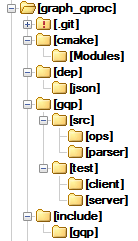
\includegraphics[scale=1]{structure}
\caption{Дерево файлов проекта}
\label{fig:structure}
\end{figure}

\lipsum[14-16]

\subsection{Руководство администратора}
\lipsum[17]

\subsection{Руководство пользователя}
\lipsum[18-19]
\newpage



\section{Тестирование системы}
\lipsum[19-21]
\clearpage



\section*{Заключение}
%\addtocontents{toc}{\protect\clearpage}
\addcontentsline{toc}{section}{Заключение}
\lipsum[23-25]
\newpage

% Список литературы
\begin{thebibliography}{00}

\bibitem{bib_name1} �������� 1

\bibitem{bib_name2} �������� 2

\bibitem{bib_name3} �������� 3

\bibitem{wiki_main} ���������: ��������� ������������: �� ������� ����� [����������� ������] // URL:  http://ru.wikipedia.org/wiki/���������\_��������  (���� ���������: 06.05.2013)

\bibitem{wiki_main} ���������: ��������� ������������: �� ������� ����� [����������� ������] // URL:  http://ru.wikipedia.org/wiki/���������\_��������  (���� ���������: \ddmmyyyydate\today)

\end{thebibliography}
\end{document}